\documentclass{article}
\usepackage[utf8]{inputenc}
\usepackage{graphicx}
\usepackage{enumitem}
\begin{document}

%%%%%%%%%%%%%%%%%%%%%%%%%%%%%%%%%%%%%%%%%%%%%%%%%%%%%%%%%%%%%%%%%%%%%%%%%%%%

\section{Uvod}
"Najmanji Problem" je ime izmišljenog ugostiteljskog objekta (kafe/klub/restoran) u Beogradu, za koji treba
konstruisati informacioni sistem, u cilju maksimizovanja profita, kroz smanjenje troškova i povećanje transparentnosti
poslovanja.\\

Moderni ugostiteljski objekti postaju sve više zavisni od informacionih tehnologija u svakodnevnom radu, dok su sa
druge strane čvrsto vezani i za zastarele oblike komunikacije i rada ukorenjene u lokalnim običajima, čineći specifičnu
mešavinu dva sveta.\\

Vodjenje ugostiteljskih objekata uključuje niz aktivnosti, čije izvršavanje može biti olakšano, ubrzano i učinjeno
transparentnim implementacijom digitalnog informacionog sistema, koji bi obezbedjivao sledeće funkcionalnosti:\\

\begin{itemize}
\item Pregled stanja zaliha namirnica i druge potrošne robe u realnom vremenu
\item Pregled inventara pribora, nameštaja i uredjaja neophodnih za funkcionisanje objekta
\item Pregled finansijskog stanja, ulaza i izlaza, kreiranje finansijskih izveštaja
\item Upravljanje ljudskim resursima (raspored godišnjih odmora, raspored smena)
\item Prihvatanje rezervacija gostiju
\item Online naručivanje i dostava hrane I pića
\item Pregled stanja trenutno aktivnih narudžbina (fizičkih i online), i izmena informacija izmedju konobara i kuhinje
\end{itemize}

Neki od podsistema su otvoreni, a neki zatvoreni, tako da postoji mogućnost demonstracije različitih tehnika razvoja
informacionih podsistema.\\

Problematika realnog sistema na kojem treba da počiva ovaj informacioni sistem je svima poznata u dovoljnoj meri,
da je moguće izvršiti inicijalno planiranje u grubim crtama, dok je za detaljniji plan neophodno terensko istraživanje.\\

Krajnji rezultat ovog projekta jeste funkcionalni prototip informacionog sistema.

%%%%%%%%%%%%%%%%%%%%%%%%%%%%%%%%%%%%%%%%%%%%%%%%%%%%%%%%%%%%%%%%%%%%%%%%%%%%

\subsection{"Najmanji problem"}

%%%%%%%%%%%%%%%%%%%%%%%%%%%%%%%%%%%%%%%%%%%%%%%%%%%%%%%%%%%%%%%%%%%%%%%%%%%%

\subsection{Moguća unapredjenja}

%%%%%%%%%%%%%%%%%%%%%%%%%%%%%%%%%%%%%%%%%%%%%%%%%%%%%%%%%%%%%%%%%%%%%%%%%%%%

\subsection{Metodologija rada}

%%%%%%%%%%%%%%%%%%%%%%%%%%%%%%%%%%%%%%%%%%%%%%%%%%%%%%%%%%%%%%%%%%%%%%%%%%%%

\subsection{Korišćeni alati}

%%%%%%%%%%%%%%%%%%%%%%%%%%%%%%%%%%%%%%%%%%%%%%%%%%%%%%%%%%%%%%%%%%%%%%%%%%%%

\section{Slučajevi upotrebe}
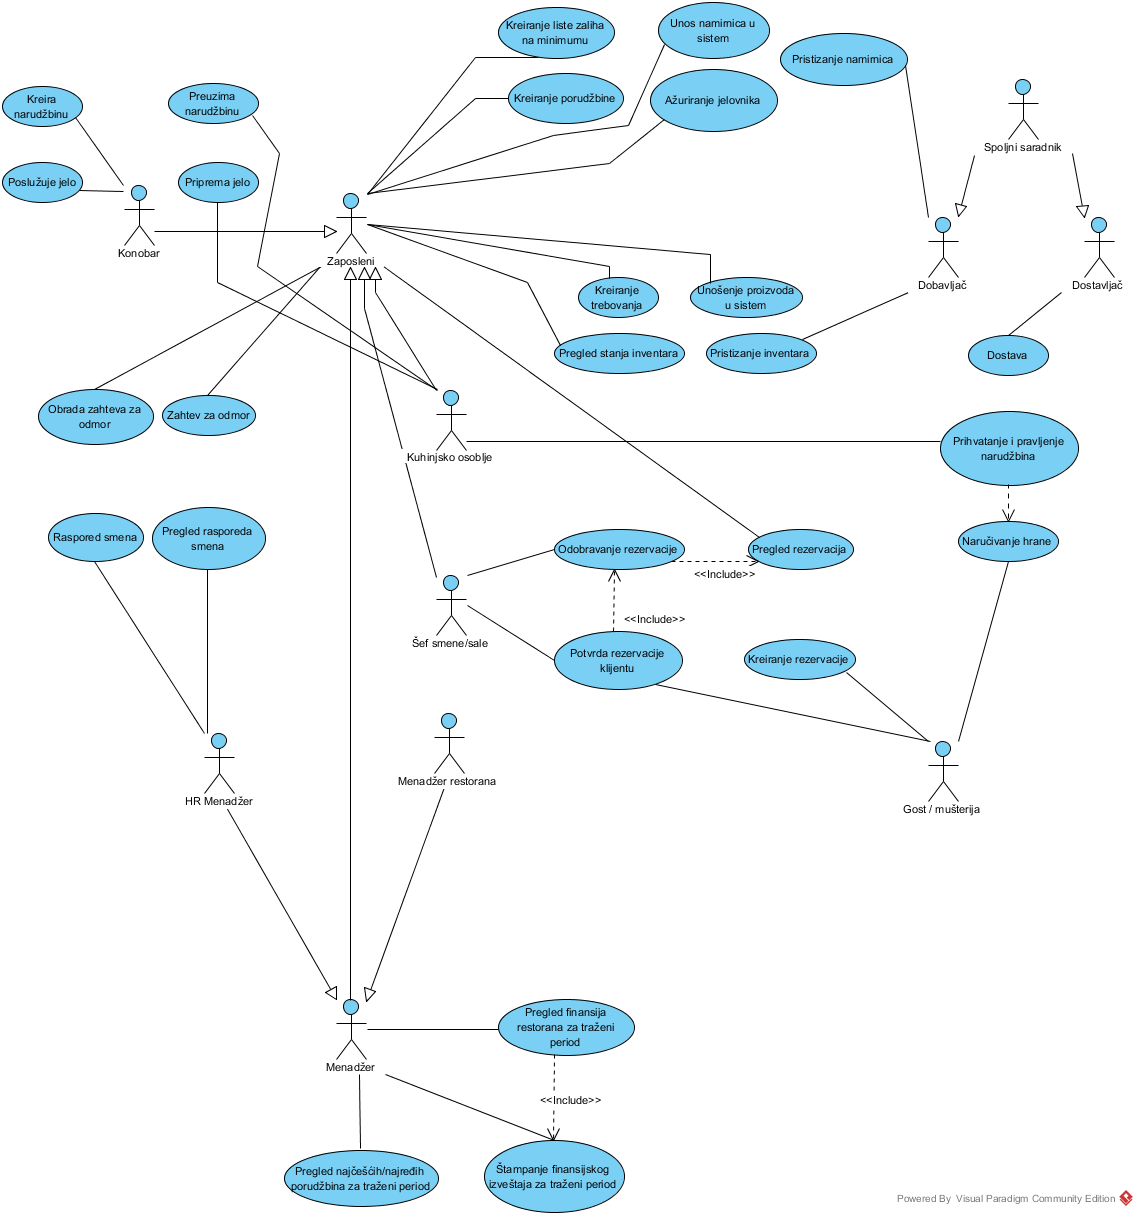
\includegraphics[width=\textwidth]{SU_0_grupni.png}
%%%%%%%%%%%%%%%%%%%%%%%%%%%%%%%%%%%%%%%%%%%%%%%%%%%%%%%%%%%%%%%%%%%%%%%%%%%%

\subsection{Zalihe namirnica}
Pregled stanja zaliha namirnica je slučaj upotrebe u kome se formalizuje način na koji ugostiteljski objekat planira nabavku namirnica, nabavlja, a potom ih dodaje na stanje. U tom procesu učestvuju menadžer nabavke (zaposleni) i dobavljač. 

\begin{itemize}
\item Zaposleni kreira spisak namirnica čija je trenutna količina ispod propisane minimalne. Na osnovu tog spiska, kreira porudžbinu. Kasnije, nakon isporuke porudžbine, unosi u bazu pristiglu robu.
\item Dobavljač isporučuje ugostiteljskom objektu namirnice u traženoj količini.
\end{itemize}
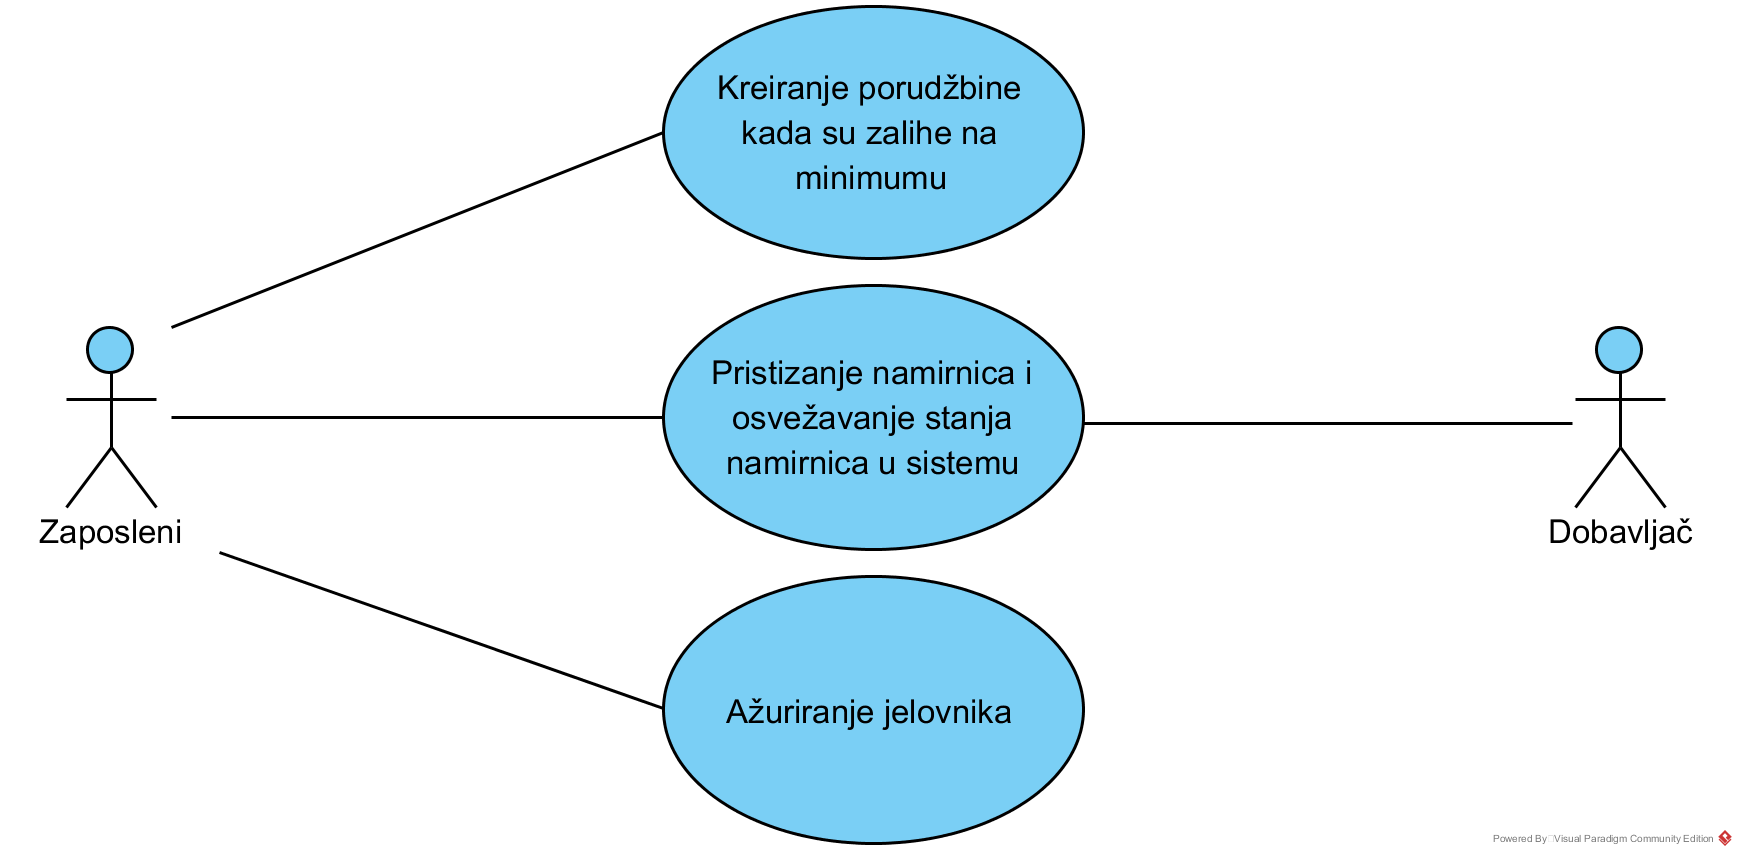
\includegraphics[width=\textwidth]{SU_1_zalihe.png}
\subsubsection{\textbf{Use Case}: Zalihe na minimumu}
\textbf{Akter:} Radnik/menadžer nabavke\\
\textbf{Ulaz:} Nema\\
\textbf{Izlaz:} Kreiran je spisak namirnica čije su zalihe na minimumu.\\
\textbf{Preduslovi:} Radnik poseduje username i lozinku za prijavljivanje na glavni sistem gde se nalaze informacije o namirnicama.\\
\textbf{Postuslov:} Uspešno je kreiran spisak namirnica.\\
\textbf{Glavni tok:} 
\begin{enumerate}
	\item Radnik se prijavljuje na sistem.
	\item Radnik zahteva od sistema spisak namirnica za koje važi da je trenutna količina manja od minimalne propisane.
	\item Sistem generiše listu namirnica koje zadovoljavaju prethodno navedeni uslov.
\end{enumerate}
\textbf{Alternativni tok:} Ukoliko ne postoji ni jedan proizvod koji ima definisanu minimalnu količinu, izveštaj o zalihama na minimumu se ne može generisati.\\

\subsubsection{\textbf{Use Case}: Kreiranje porudžbine}
\textbf{Akter:} Radnik/menadžer nabavke\\
\textbf{Ulaz:} Lista namirnica čije su zalihe na minimumu.\\
\textbf{Izlaz:} Lista poručenih namirnica.\\
\textbf{Preduslovi:} Radnik ima uvid u spisak namirnica čija je količina manja od poželjne.\\
\textbf{Postuslov:} Porudžbina je kreirana.\\
\textbf{Glavni tok:} 
\begin{enumerate}
	\item Radnik uzima listu namirnica koje bi trebalo nabaviti.
	\item Za svaku namirnicu procenjuje količinu za nabavku. 
	\item Na spisak može dodati i namirnice kojih nema i nikada ih nije bilo u sistemu. 
	\item Kreira porudžbinu.
\end{enumerate}
\textbf{Alternativni tok:} Ukoliko je lista namirnica na minimalnim zalihama prazna, procena se ne vrši.\\

\subsubsection{\textbf{Use Case}:  Pristizanje namirnica}
\textbf{Akter:} Dobavljač\\
\textbf{Ulaz:} Lista poručenih namirnica.\\
\textbf{Izlaz:} Lista namirnica koje je dobavljač isporučio ugostiteljskom objektu.\\
\textbf{Preduslovi:} Dobavljač je dobio porudžbinu.\\
\textbf{Postuslov:} Namirnice su isporučene kupcu i kreirana je lista dostavljenih proizvoda.\\
\textbf{Glavni tok:} 
\begin{enumerate}
	\item Dobavljač je primio porudžbinu.
	\item Procenjuje da li je njegva firma u mogućnosti da odgovori na zahteve ugostiteljskog objekta, ukoliko nije, otkazuje porudžbinu.
	\item Za svaku namirnicu odlučuje da li će isporučiti u smanjenoj ili traženoj količini.
	\item Isporučuje robu ugostiteljskom objektu.
	\item Pri isporuci dostavljena je lista namirnica koje su isporučene.
\end{enumerate}
\textbf{Alternativni tok:} Zbog manjka raspoloživih namirnica, dobavljač otkazuje porudžbinu.\\

\subsubsection{\textbf{Use Case}: Unos namirnica u sistem}
\textbf{Akter:} Radnik\\
\textbf{Ulaz:} Spisak namirnica koje je dobavljač isporučio.\\
\textbf{Izlaz:} Ažurirana je lista namirnica.\\
\textbf{Preduslovi:} Radnik poseduje username i lozinku za prijavljivanje na glavni sistem. Dobavljač je dostavio poručene namirnice.\\
\textbf{Postuslov:} Ažurirane su količine namirnica i eventualno unete nove.\\
\textbf{Glavni tok:} 
\begin{enumerate}
	\item Radnik je dobio listu isporučenih namirnica.
	\item Radnik se prijavljuje na sistem.
	\item Za svaki od proizvoda sa liste, radnik ažurira proizvod u sistemu tako što dodaje pristiglu količinu.
	\item Ukoliko proizvod ne postoji u sistemu, radnik kreira novi.
	\item Ažurira novokreiranu namirnicu pristiglom količinom i eventualno definiše minimalnu količinu. 
\end{enumerate}
\textbf{Alternativni tok:} Porudžbina je otkazana od strane dobavljača, nema unosa.\\

\subsubsection{\textbf{Use Case}: Ažuriranje jelovnika}
\textbf{Akter:} Radnik\\
\textbf{Ulaz:} Spisak namirnica u restoranu i spisak jela sa neophodnim namirnicama za njihovu pripremu.\\
\textbf{Izlaz:} Kreiran je jelovnik.\\
\textbf{Preduslovi:} Radnik poseduje username i lozinku za prijavljivanje na glavni sistem. Spisak jela i sastojaka od kojih se pripremaju nije prazan.\\
\textbf{Postuslov:} Jelovnik je kreiran. Gosti i zaposleni ga mogu videti.\\
\textbf{Glavni tok:} 
\begin{enumerate}
	\item Radnik zahteva od sistema ažuriranje jelovnika.
	\item Sistem na njegov zahtev kreira novi jelovnik tako što iz liste jela izbacuje ona za čiju pripremu nedostaje makar jedan sastojak.
	\item Kreirani jelovnik postaje aktuelni jelovnik ugostiteljskog objekta.
\end{enumerate}
\textbf{Alternativni tok:} Ne postoje podaci koji povezuju jela i namirnice, novi jelovnik se ne može generisati. Aktuelni jelovnik se ne ažurira.\\
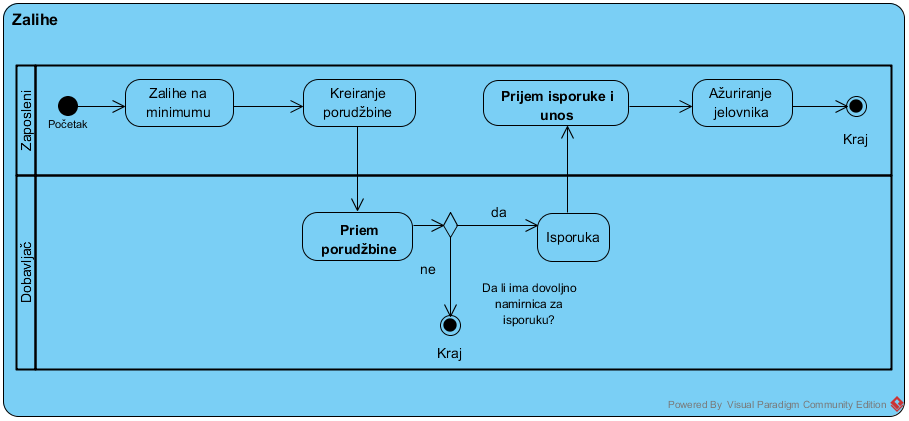
\includegraphics[width=\textwidth]{SU_1_zalihe_activity.png}

%%%%%%%%%%%%%%%%%%%%%%%%%%%%%%%%%%%%%%%%%%%%%%%%%%%%%%%%%%%%%%%%%%%%%%%%%%%%

\subsection{Pregled inventara}
Pregled inventara je slučaj upotrebe u kome se formalizuje način na koji ugostiteljski objekat planira nabavku inventara, nabavlja i ima uvid o stanju istog. U tom procesu učestvuju radnik i dobavljač. 

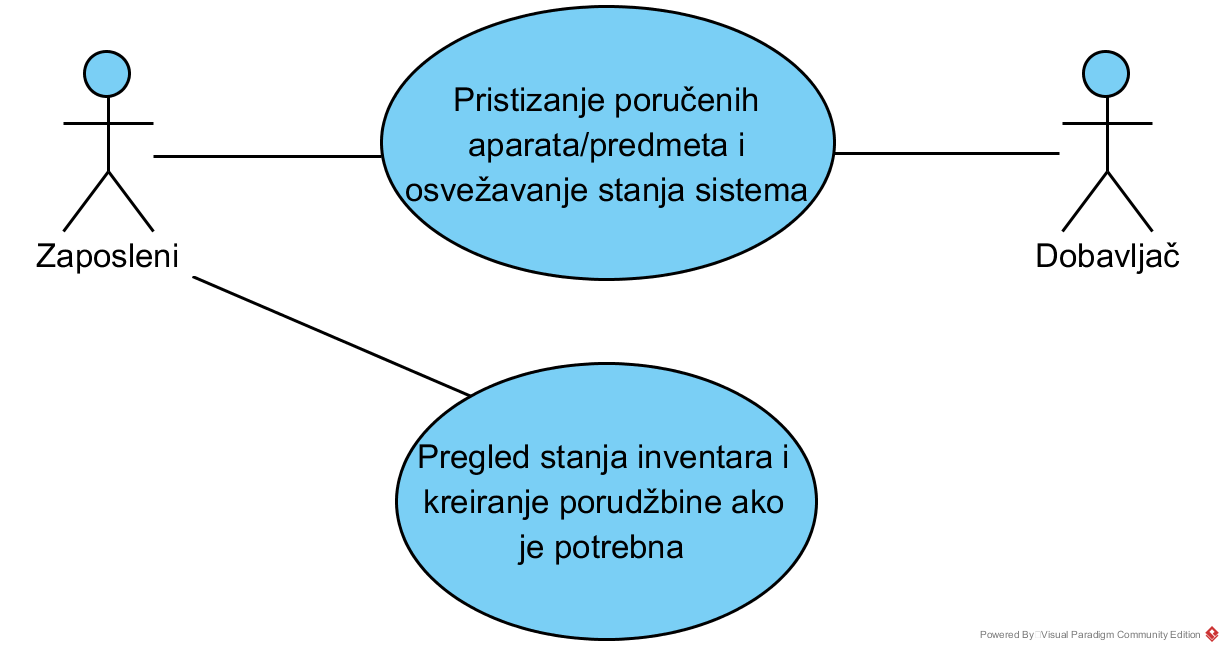
\includegraphics[width=\textwidth]{SU_2_pregled_inventara.png}
\subsubsection{\textbf{Use Case}: Pregled stanja inventara}
\textbf{Akter:} Zaposleni restorana\\
\textbf{Ulaz:} Nema\\
\textbf{Izlaz:} 
\begin{enumerate}
	\item Spisak predmeta koji spadaju u inventar ugostiteljskog objekta i njihove zalihe su usled kvara ili nestanka ispod minimalnih definisanih količina.
	\item Lista svih predmeta i njihova trenutna količina.
\end{enumerate} 
\textbf{Preduslovi:} Radnik se uspešno ulogovao na sistem.\\
\textbf{Postuslov:} Uspešno je kreiran spisak predmeta. Ukoliko neki predmet zahteva popravku, lista sadrži tu informaciju.\\
\textbf{Glavni tok:} 
\begin{enumerate}
	\item Radnik se prijavljuje na sistem.
	\item Zahteva od  od sistema spisak predmeta za koje važi da je trenutna količina manja od minimalne propisane ili je neki od aparata u kvaru.
	\item Sistem kreira listu predmeta koji ispunjavaju prethodni zahtev.
\end{enumerate}
\textbf{Alternativni tok:} Ne postoje podaci o minimalnim količinama ni za jedan predmet u sistemu, pa nije moguće kreirati pregled stanja.\\

\subsubsection{\textbf{Use Case}: Kreiranje porudžbine}
\textbf{Akter:} Zaposleni restorana\\
\textbf{Ulaz:} Lista predmeta čije su zalihe ispod minimalnih definisanih za poslovanje ugostiteljskog objekta.\\
\textbf{Izlaz:} Lista poručenih predmeta.\\
\textbf{Preduslovi:} Radnik ima uvid u spisak predmeta čija je količina manja od poželjne.\\
\textbf{Postuslov:} Porudžbina je kreirana.\\
\textbf{Glavni tok:} 
\begin{enumerate}
	\item Radnik uzima listu predmeta koje bi trebalo nabaviti.
	\item Radnik procenjuje količinu za nabavku. 
	\item Radnik proverava da li postoje predmeti koje želi da uvrsti u inventar i doda ih u porudžbinu.
	\item Kreira porudžbinu.
\end{enumerate}
\textbf{Alternativni tok:} Ukoliko je lista predmeta na minimalnim zalihama prazna, procena količina se ne vrši.\\

\subsubsection{\textbf{Use Case}:  Pristizanje predmeta i aparata}
\textbf{Akter:} Dobavljač\\
\textbf{Ulaz:} Lista poručenih predmeta.\\
\textbf{Izlaz:} Lista predmeta koje je dobavljač isporučio ugostiteljskom objektu.\\
\textbf{Preduslovi:} Dobavljač je dobio porudžbinu.\\
\textbf{Postuslov:} Predmeti su isporučeni kupcu i kreirana je lista dostavljenih proizvoda.\\
\textbf{Glavni tok:} 
\begin{enumerate}
	\item Dobavljač je dobio listu poručenih proizvoda.
	\item Proverava za svaki proizvod da li je njegova firma u mogućnosti da isporuči tražene količine.
	\item Po potrebi, smanjuje količine koje su poručene.
	\item Isporučuje robu ugostiteljskom objektu.
	\item Pri isporuci dostavljena je lista predmeta koji su isporučeni.
\end{enumerate}
\textbf{Alternativni tok:} Zbog manjka raspoloživih predmeta, dobavljač otkazuje porudžbinu.\\

\subsubsection{\textbf{Use Case}: Unos predmeta u sistem}
\textbf{Akter:} Radnik\\
\textbf{Ulaz:} Spisak predmeta koje je dobavljač isporučio.\\
\textbf{Izlaz:} Ažurirana je lista predmeta koji čine inventar.\\
\textbf{Preduslovi:} Radnik se uspešno ulogovao na sistem. Dobavljač je dostavio poručene proizvode.\\
\textbf{Postuslov:} Ažurirane su količine proizvoda i eventualno uneti novi.\\
\textbf{Glavni tok:} 

\begin{enumerate}
	\item Radnik je dobio listu isporučenih proizvoda.
	\item Radnik se prijavljuje na sistem.
	\item Za svaki od proizvoda sa liste, radnik ažurira proizvod u sistemu tako što dodaje pristiglu količinu.
	\item Ukoliko proizvod ne postoji u sistemu, radnik kreira proizvod sa njegovim karakteristikama.
	\item Ažurira novokreirani proizvod pristiglom količinom i eventualno definiše minimalnu količinu. 
\end{enumerate}
\textbf{Alternativni tok:} Porudžbina je otkazana, nema unosa.\\


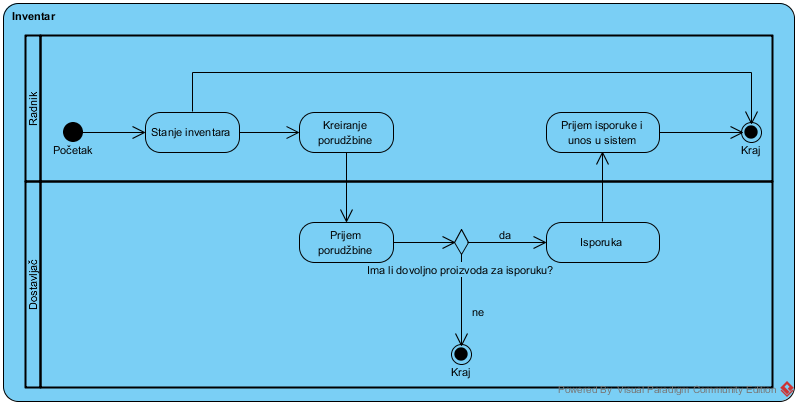
\includegraphics[width=\textwidth]{SU_2_pregled_inventara_activity.png}

%%%%%%%%%%%%%%%%%%%%%%%%%%%%%%%%%%%%%%%%%%%%%%%%%%%%%%%%%%%%%%%%%%%%%%%%%%%%

\subsection{Pregled finansijskog stanja}
Pregled finansijskog stanja je slučaj upotrebe u kojem menadžer restorana ima mogućnost pregleda prihoda i rashoda za dati vremenski period, koji se izračunavaju na osnovu naplaćenih usluga i troškova nabavke, održavanja, prihoda zaposlenih, itd.
\\
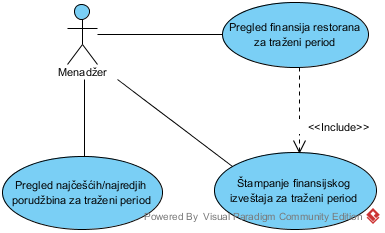
\includegraphics[width=\linewidth]{SU_3_pregled_finansija.png}

\subsubsection{\textbf{Use Case}: Pregled finansija restorana za traženi period}
\textbf{Akter:} Menadžer\\
\textbf{Ulaz:} Datum početka perioda od interesa, datum kraja perioda od interesa\\
\textbf{Izlaz:} Tabelarni prikaz prihoda i rashoda za traženi period\\
\textbf{Preduslovi:} Menadžer ima pravo pristupa stranici za pregled finansija, svi navedeni datumi su ispravni, restoran je imao barem jedan poslovni dan u navedenom periodu.\\
\textbf{Postuslov:} Nema\\
\textbf{Glavni tok:}
\begin{enumerate}
\item Korisnik unosi korisničko ime i lozinku
\item Korisnik se prijavljuje na sistem
\item Korisnik vrši odabir početnog i krajnjeg dana perioda od interesa
\item Korisnik dobija spisak prihoda i rashoda u datom vremenskom periodu.
\end{enumerate}
\textbf{Alternativni tok:} \\
        2.1. Prijavljivanje nije uspešno, korisnik se preusmerava na poruku sa greškom.\\
        3.1. Uneti datumi nisu validni, korisnik se moli da ponovo unese datume i nastavlja na koraku 3.\\
        3.2. Za unete datume, restoran nije imao nijedan poslovni dan, prikazuje se adekvatna poruka na ekranu i korisnik se preusmerava nazad na korak 3.\\
		
\subsubsection{\textbf{Use Case}: Štampanje finansijskog izveštaja za traženi period}
\textbf{Akter:} Menadžer\\
\textbf{Ulaz:} Datum početka perioda od interesa, datum kraja perioda od interesa, način štampanja.\\
\textbf{Izlaz:} Tabelarni prikaz prihoda i rashoda za traženi period i .pdf verzija finansijskog izveštaja.\\
\textbf{Preduslovi:} Menadžer ima pravo pristupa stranici za pregled finansija, svi navedeni datumi su ispravni, restoran je imao barem jedan poslovni dan u navedenom periodu, postoji barem jedan štampač povezan na sistem.\\
\textbf{Postuslov:} Odštampan finansijski izveštaj ima identične podatke kao i prikazani.\\
\textbf{Glavni tok:}
\begin{enumerate}
\item Korisnik unosi korisničko ime i lozinku
\item Korisnik se prijavljuje na sistem
\item Korisnik vrši odabir početnog i krajnjeg dana perioda od interesa
\item Korisnik dobija spisak prihoda i rashoda u datom vremenskom periodu
\item Korisniku se prikazuje dijalog za štampu kreiranog izveštaja za navedeni period.
\end{enumerate}
\textbf{Alternativni tok:}\\
        2.1. Prijavljivanje nije uspešno, korisnik se preusmerava na poruku sa greškom.\\
        3.1. Uneti datumi nisu validni, korisnik se moli da ponovo unese datume i nastavlja na koraku 3.\\
        3.2. Za unete datume, restoran nije imao nijedan poslovni dan, prikazuje se adekvatna poruka na ekranu i korisnik se preusmerava nazad na korak 3.\\
        5.1 Nijedan štampač nije povezan na sistem, prikazuje se poruka o grešci.
       
\subsubsection{\textbf{Use Case}: Pregled najčešćih/najredjih porudžbina za traženi period.}
\textbf{Akter:} Menadžer\\
\textbf{Ulaz:} Datum početka perioda od interesa, datum kraja perioda od interesa.\\
\textbf{Izlaz:} Lista stavki sa menija koje su najčešće/najredje naručivane u traženom periodu.\\
\textbf{Preduslovi:} Menadžer ima pravo pristupa stranici za pregled finansija, svi navedeni datumi su ispravni, restoran je imao barem jedan poslovni dan u navedenom periodu.\\
\textbf{Postuslov:} Nema.\\
\textbf{Glavni tok:}
\begin{enumerate}
\item Korisnik unosi korisničko ime i lozinku
\item Korisnik se prijavljuje na sistem
\item Korisnik vrši odabir početnog i krajnjeg dana perioda od interesa
\item Korisnik dobija spisak najčešće i najredje naručivanih stavki sa menija.
\end{enumerate}
\textbf{Alternativni tok:}\\
        2.1. Prijavljivanje nije uspešno, korisnik se preusmerava na poruku sa greškom.\\
        3.1. Uneti datumi nisu validni, korisnik se moli da ponovo unese datume i nastavlja na koraku 3.\\
        3.2. Za unete datume, restoran nije imao nijedan poslovni dan, prikazuje se adekvatna poruka na ekranu i korisnik se preusmerava nazad na korak 3.\\

%%%%%%%%%%%%%%%%%%%%%%%%%%%%%%%%%%%%%%%%%%%%%%%%%%%%%%%%%%%%%%%%%%%%%%%%%%%%

\subsection{Upravljanje ljudskim resursima}
Upravljanje ljudskim resursima je slučaj upotrebe u kojem se definišu rasporedi smena i godišnjih odmora. U planiranju učestvuju radnik i (hr)menadžer.

\begin{itemize}
\item Radnik svoje želje za godišnjim odmorom predaje na odobravanje menadžeru koji te želje skuplja, obradjuje, planira i na kraju daje pozitivan ili negativan odgovor.
\item Raspored smena pravi menažer, koji su potom dostupni na pregled radnicima.
\end{itemize}
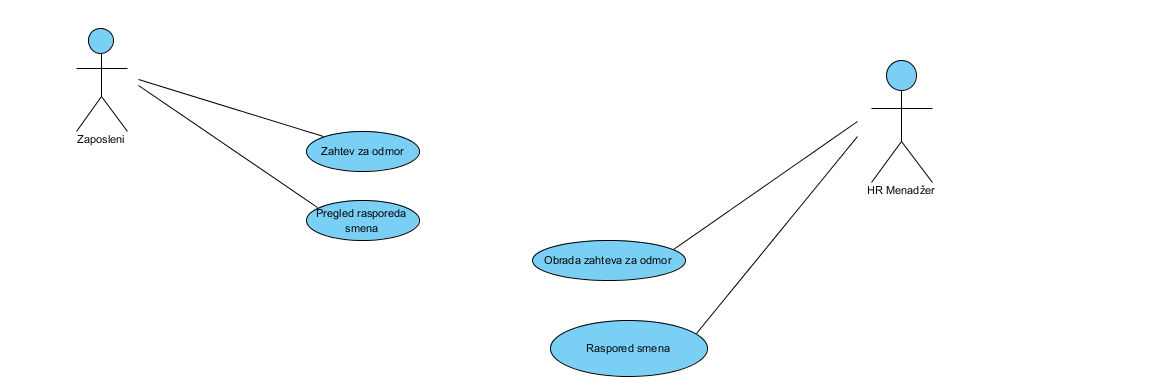
\includegraphics[width=\textwidth]{SU_4_hr.png}
\subsubsection{\textbf{Use Case}: Zahtev za odmor}
\textbf{Akter:} Radnik\\
\textbf{Ulaz:} Nema\\
\textbf{Izlaz:} Definisan zahtev za odmor\\
\textbf{Preduslovi:} Radnik poseduje username i lozinku za prijavljivanje na glavni sistem gde se definišu zahtevi\\
\textbf{Postuslov:} Uspešno poslat zahtev za odmor\\
\textbf{Glavni tok:} Radnik na osnovu svojih potreba i želja šalje zahtev za godišnji odmor putem glavnog sistema, gde definiše početak i kraj odmora.\\
\textbf{Alternativni tok:} Prijavljivanje nije uspešno, zahtev se ne može napraviti\\

\subsubsection{\textbf{Use Case}: Obrada zahteva za odmor}
\textbf{Akter:} Menadžer\\
\textbf{Ulaz:} Spiskovi zahteva za odmor\\
\textbf{Izlaz:} Definisani odgovori na zahteve\\
\textbf{Preduslovi:}Menadžer se uspešno ulogovao na sistem i spiskovi zahteva su uspešno stigli do njega\\
\textbf{Postuslov:} Odgovori su definisani\\
\textbf{Glavni tok:} Menadžer uzima spiskove zahteva za odmor i procenjuje ukoliko radnici imaju dovoljan broj preostalih slobodnih dana, da li je moguće organizovati funkcionisanje restorana u datom periodu bez dotičnog radnika, da li je zakonom definisano da radnik mora uzeti odmor(npr. ukolko mu je ostao odmor od prethodne godine). Na osnovu procene stanja donosi se odluka.
\textbf{Alternativni tok:} Ukoliko su navedeni zahtevi za slobodnim danima definisani zakonom(slava, selidba, smrtni slučaj, rodjenje deteta,..) dani se odobravaju bez dodatnih procena\\
\subsubsection{\textbf{Use Case}: Raspored smena}
\textbf{Akter:} Menadžer\\
\textbf{Ulaz:} Nema\\
\textbf{Izlaz:} Novi raspored smena za odredjeni period\\
\textbf{Preduslovi:} Postoje informacije o planu rada restorana za dati period kao i spisak godišnjih odmora\\
\textbf{Postuslov:}Sastavjen je novi raspored smena za odredjeni period i spreman je za slanje\\
\textbf{Glavni tok:} Menadžer definiše rasporede smena, za odredjeni period, na osnovu plana rada restorana i definisanih godišnjih odmora\\
\textbf{Alternativni tok:} Zbog promene plana rada restorana ili odsustva radnika, već postojeći raspored mora da se menja\\

\subsubsection{\textbf{Use Case}: Pregled rasporeda smena}
\textbf{Akter:} Radnik\\
\textbf{Ulaz:} Nema\\
\textbf{Izlaz:} Raspored smena za radnika\\
\textbf{Preduslovi:} Radnik poseduje username i lozinku za prijavljivanje na glavni sistem\\
\textbf{Postuslov:} Uspešan pregled smena\\
\textbf{Glavni tok:}Radnik može da vidi svoj raspored smena i u skladu sa tim da dolazi na posao\\
\textbf{Alternativni tok:}Još nije definian raspored smena za željeni period, radnik nema šta da vidi\\
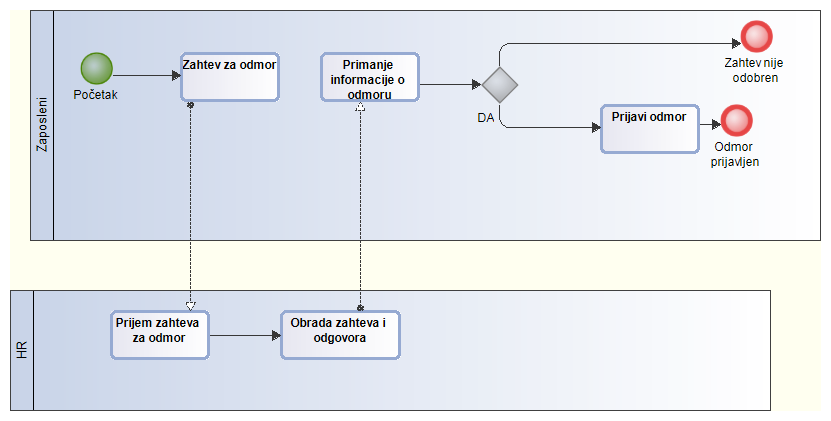
\includegraphics[width=\textwidth]{SU_4_Odmor.png}\\
\includegraphics[width=\textwidth]{SU_4_Raspored_smena.png}\\

%%%%%%%%%%%%%%%%%%%%%%%%%%%%%%%%%%%%%%%%%%%%%%%%%%%%%%%%%%%%%%%%%%%%%%%%%%%%

\subsection{Prihvatanje rezervacija gostiju}
"Prihvatanje rezervacija gostiju" je slučaj upotrebe u kojem se vrši prihvat i obrada digitalnih rezervacija mesta u restoranu. U tom procesu učestvuju potencijalni gost restorana, šef smene/sale restorana, kao i ostali zaposleni.

\begin{itemize}
\item Potencijalni gost restorana posećuje stranicu za digitalne rezervacije i unosi sve potrebne podatke za rezervaciju
\item Šef smene ili sale odobrava rezervaciju na osnovu pregleda prethodno unetih rezervacija i potvrdjuje(ili odbija) rezervaciju potencijalnom gostu.
\end{itemize}
\vspace{1cm}
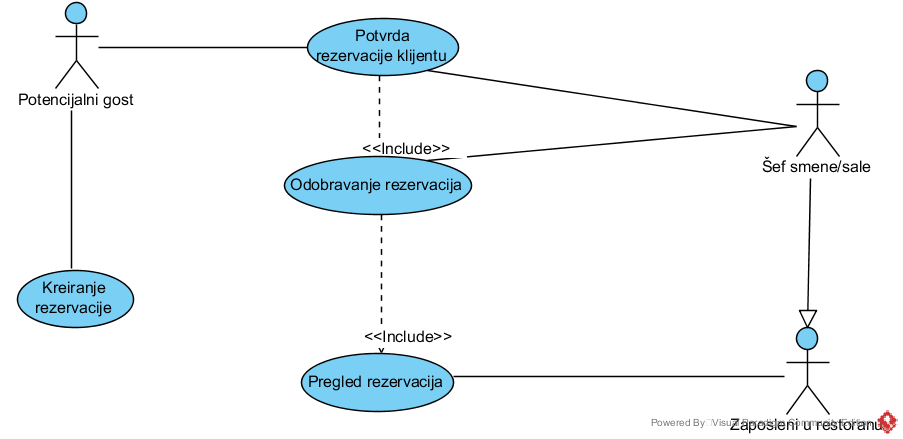
\includegraphics[width=\textwidth]{SU_5_prihvatanje_rezervacija.png}

\subsubsection{\textbf{Use Case}: Kreiranje rezervacije}
\textbf{Akter:} Potencijalni gost restorana\\
\textbf{Ulaz:} Kontakt podaci potencijalnog gosta (ime, prezime, kontakt telefon ili e-mail adresa), datum rezervacije, broj gostiju, specijalne napomene\\
\textbf{Izlaz:} Redni broj zahteva za rezervaciju.\\
\textbf{Preduslovi:} Nema.\\
\textbf{Postuslov:} Uspešno je kreiran zahtev za rezervaciju.\\
\textbf{Glavni tok:}
\begin{enumerate}
\item Korisnik vrši navigaciju na stranu za rezervaciju
\item Korisnik unosi zahtevane podatke
\item Korisnik šalje restoranu zahtev za rezervaciju
\item Korisnik dobija potvrdu da je zahtev za rezervaciju dostavljen restoranu na obradu.\\
\end{enumerate}
\textbf{Alternativni tok:}\\
		4.1.1 Potvrda o poslatom zahtevu ne stiže u roku od 2 minuta\\
		4.1.2 Prikazuje se izvinjenje i kontakt telefon kojim se može izvršiti rezervacija "offline".\\

\subsubsection{\textbf{Use Case}: Pregled rezervacija}
\textbf{Akter:} Zaposleni restorana\\
\textbf{Ulaz:} Datum i/ili broj stola za koji se pregleda spisak rezervacija.\\
\textbf{Izlaz:} Spisak registrovanih rezervacija koje odgovaraju kriterijumu pretrage.\\
\textbf{Preduslovi:} Zaposleni ima pristup glavnom sistemu.\\
\textbf{Postuslov:} Nema.\\
\textbf{Glavni tok:}
\begin{enumerate}
\item Korisnik unosi korisničko ime i lozinku
\item Korisnik se prijavljuje na sistem
\item Korisnik unosi ulazne parametre
\item Korisnik dobija tabelarni prikaz registrovanih rezervacija koje zadovoljavaju kriterijume pretrage.\\
\end{enumerate}
\textbf{Alternativni tok:}\\
        2.1. Prijavljivanje nije uspešno, korisnik se preusmerava na poruku sa greškom.\\

\subsubsection{\textbf{Use Case}:  Odobravanje rezervacija}
\textbf{Akter:} Šef smene/sale\\
\textbf{Ulaz:} Podaci iz pristiglog zahteva za rezervaciju, informacije o već registrovanim rezervacijama i raspoloživom broju i strukturi mesta.\\
\textbf{Izlaz:} Rezervacija odobrena ili odbijena i redni broj rezervacije.\\
\textbf{Preduslovi:} Postoji barem jedan neobradjen zahtev za rezervaciju i trenutni korisnik sistema ima pravo da pristupi odobravanju rezervacija.\\
\textbf{Postuslov:} Informacije o odobrenim rezervacijama su sačuvane u sistemu.\\
\textbf{Glavni tok:}
\begin{enumerate}
\item Korisnik unosi korisničko ime i lozinku
\item Korisnik se prijavljuje na sistem
\item Korisnik pregleda spisak dospelih zahteva za rezervaciju
\item Korisnik za svaki od zahteva vrši pregled rezervacija da bi utvrdio da li je rezervacija sa zadatim parametrima moguća
\item Korisnik odobrava ili odbija rezervaciju i svoju odluku registruje u sistemu.\\
\end{enumerate}
\textbf{Alternativni tok:}\\
       2.1. Prijavljivanje nije uspešno, korisnik se preusmerava na poruku sa greškom.\\

\subsubsection{\textbf{Use Case}: Uklanjanje registrovanih rezervacija}
\textbf{Akter:} Šef smene/sale\\
\textbf{Ulaz:} Redni broj rezervacija koju treba obrisati i razlog brisanja.\\
\textbf{Izlaz:} Nema.\\
\textbf{Preduslovi:} Trenutni korisnik ima pravo da pristupi meniju za uklanjanje registrovanih rezervacija. Postoji validan razlog za uklanjanje rezervacije koji je iskomuniciran sa klijentom (sa čije god strane da je razlog potekao).\\
\textbf{Postuslov:} Rezervacija sa datim rednim brojem je uklonjena iz sistema i razlog uklanjanja je registrovan.\\
\textbf{Glavni tok:}
\begin{enumerate}
\item Korisnik unosi korisničko ime i lozinku
\item Korisnik se prijavljuje na sistem
\item Korisnik unosi ulazne podatke
\item Rezervacija se uklanja iz sistema
\item Korisniku se prikazuju preostale rezervacije za dan uklonjene rezervacije.\\
\end{enumerate}
\textbf{Alternativni tok:}\\
       2.1. Prijavljivanje nije uspešno, korisnik se preusmerava na poruku sa greškom.\\
	   4.1. Rezervacija sa datim rednim brojem ne postoji u sistemu. Korisniku se prijavljuje greška i prikazuje se spisak poslednjih deset uklonjenih rezervacija.\\

\subsubsection{\textbf{Use Case}: Potvrda rezervacije klijentu}
\textbf{Akter:} Šef smene/sale, potencijalni gost restorana.\\
\textbf{Ulaz:} Redni broj rezervacije i kontakt podaci potencijalnog gosta.\\
\textbf{Izlaz:} Rezervacija je potvrdjena ili ne.\\
\textbf{Preduslovi:} Trenutni korisnik ima pravo da pristupi meniju za potvrdjivanje rezervacija, kontakt podaci potencijalnog gosta su validni.\\
\textbf{Postuslov:} Rezervacija je potvrdjena.\\
\textbf{Glavni tok:}
\begin{enumerate}
\item Korisnik unosi korisničko ime i lozinku
\item Korisnik se prijavljuje na sistem
\item Korisnik pregleda odabranu rezervaciju
\item Korisnik šalje potvrdu gostu automatski generisanom elektronskom poštom ili poziva gosta telefonom.\\
\end{enumerate}
\textbf{Alternativni tok:}\\
       2.1. Prijavljivanje nije uspešno, korisnik se preusmerava na poruku sa greškom.\\
       4.1. Kontakt podaci nisu validni, rezervacija se automatski registruje kao uklonjena, sa razlogom "nevalidni kontakt podaci gosta".\\

%%%%%%%%%%%%%%%%%%%%%%%%%%%%%%%%%%%%%%%%%%%%%%%%%%%%%%%%%%%%%%%%%%%%%%%%%%%%

\subsection{Online naručivanje i dostava hrane i pića}
Online naručivanje i dostava hrane i pića je slučaj upotrebe gde mušterija definiše svoju narudžbinu, radnici je prave, a dostavljači isporučuju. U naručivaju učestvuju: mušterija, radnik i dostavljač.
\\
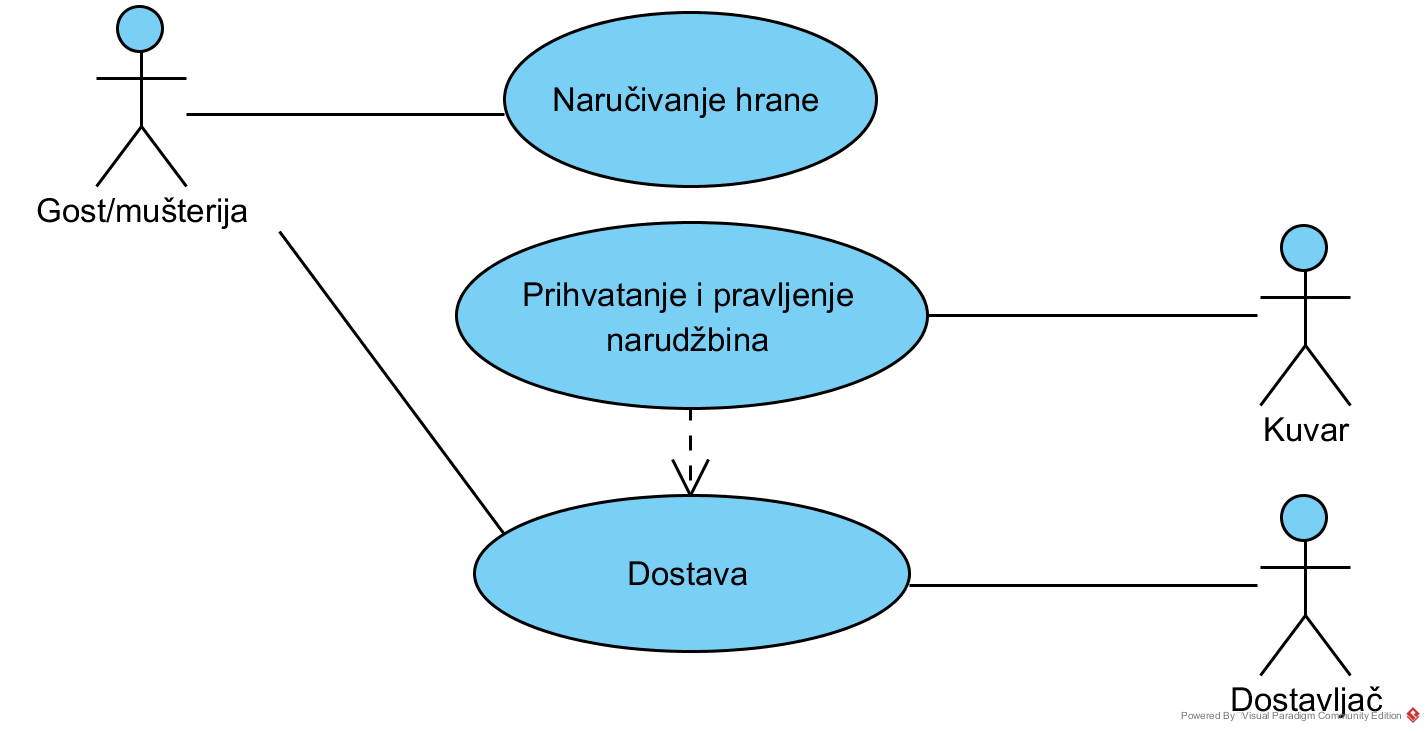
\includegraphics[width=\linewidth]{SU_6_dostava.png}

\subsubsection{\textbf{Use Case}: Pravljenje narudžbine}
\textbf{Akter:} Mušterija\\
\textbf{Ulaz:} Nema\\
\textbf{Izlaz:} Definisana narudžbina\\
\textbf{Preduslovi:} Restoran prima narudžbine\\
\textbf{Postuslov:} Uspešno napravljena narudžbina je poslata restoranu\\
\textbf{Glavni tok:}
\begin{enumerate}
\item Ukoliko mušterija nema nalog na sistemu, vrši registraciju i dobija korisničko ime i lozinku od sistema
\item Mušterija unosi korisničko ime i lozinku
\item Mušterija se prijavljuje na sistem
\item Mušterija vrši odabir hrane i pića
\item Mušterija ostavlja podatke o adresi za dostavu
\item Mušerija potvrdjuje narudžbinu, koja se dalje prosledjuje na sistem
\end{enumerate}
\textbf{Alternativni tok:} \\
        3.1. Prijavljivanje nije uspešno, mušterija se vraća na korak 2\\


\subsubsection{\textbf{Use Case}: Prihvatanje i pravljenje narudžbina}
\textbf{Akter:} Radnik, Dostavljač\\
\textbf{Ulaz:} Spisak narudžbina\\
\textbf{Izlaz:} Napravljene narudžbine\\
\textbf{Preduslovi:} Radnik se uspešno ulogovao na sistem i spiskovi narudžbina su uspešno stigli do njega\\
\textbf{Postuslov:}  Napravljene narudžbine su spremne za dostavu\\
\textbf{Glavni tok:}
\begin{enumerate}
\item Radnik uzima spiskove narudžbina
\item Za svaku narudžbinu iz spiska pravi se porcija, po redosledu vremena naručivanja
\item Po završetku pravljenja obroka, radnik obaveštava Dostavljača da je porudžbina spremna za dostavu 
\end{enumerate}
\textbf{Alternativni tok:}\\
       2.1. Ukoliko  fale sastojci za neku od narudžbina, prelazi se na sedeću narudžbinu dok sastojci ne stignu\\
       
       
\subsubsection{\textbf{Use Case}: Dostava i prihvatanje dostave}
\textbf{Akter:} Dostavljač, Mušterija\\
\textbf{Ulaz:} Pripremljena narudžbina\\
\textbf{Izlaz:} Izvršena dostava\\
\textbf{Preduslovi:} Mušterija je ispravno definisala adresu\\
\textbf{Postuslov:}  Izvršena dostava je plaćena\\
\textbf{Glavni tok:}
\begin{enumerate}
\item Dostavljač odnosi porudžbina na adresu definisanu na narudžbini
\item Mušterija prihvata porudžbinu i proverava da li je sve u redu sa sadržajem
\item Mušterija plaća dostavu
\end{enumerate}
\textbf{Alternativni tok:}\\
       2.1 Ukoliko nije sve u redu sa sadržajem, pravi se nova narudžbna i mušterija čeka novu dostavu, ili mušterija odustaje od narudžbine\\
       2.2 Ukoliko je mušterija odustala, dostavljač vraća hranu u restoran

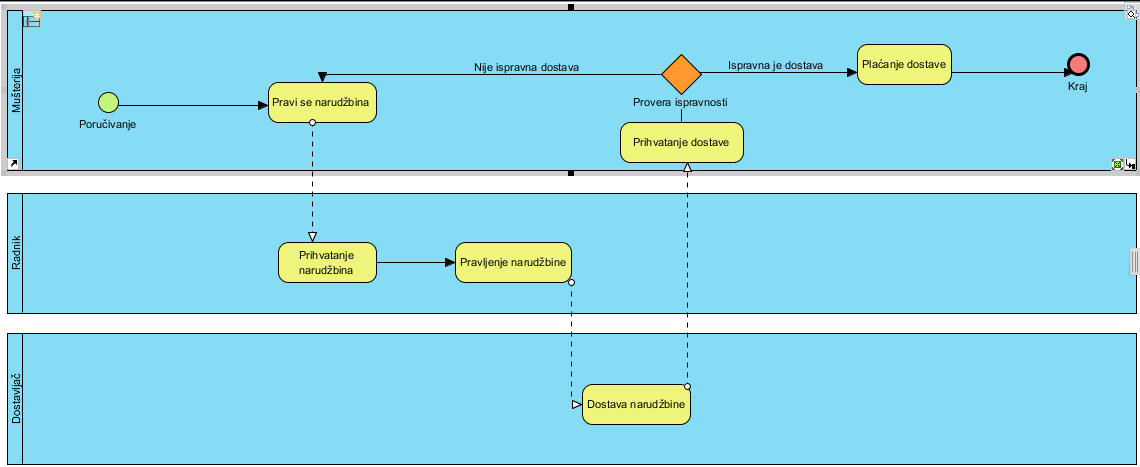
\includegraphics[width=\textwidth]{SU_6_dostava_bpmn.png}

%%%%%%%%%%%%%%%%%%%%%%%%%%%%%%%%%%%%%%%%%%%%%%%%%%%%%%%%%%%%%%%%%%%%%%%%%%%%

\subsection {Obrada porudžbine gosta}

Porudžbina je niz slučajeva upotrebe u kojima se formalizuje komunikacija 3 učesnika - gosta, konobara i kuhinje, tokom života jedne porudžbine. Ova porudžbina može biti preko onlajn servisa, ili direktno preko konobara.

\subsubsection{\textbf{Use Case}: Gost poručuje jelo}
\textbf{Akteri:} Gost kafane, konobar
\textbf{Ulaz:} Jelovnik.
\textbf{Izlaz:} Porudžbina.
\textbf{Preduslov:} Gost je u kafani.
\textbf{Postuslov:} Uspešno je napravljen skup porudzbina gosta.
\textbf{Glavni tok:} Gost potrazuje jelo sa menija, i konobar uspesno beleži narudžbinu
\textbf{Alternativni tok:} Gost je nezadovoljan zbog dugog čekanja konobara

\subsubsection{\textbf{Use Case:} Konobar prenosi porudžbinu kuhinji}
\textbf{Akteri:} Konobar
\textbf{Ulaz:} Jelovnik
\textbf{Izlaz:} Osvežen globalni spisak porudžbina kojim se vodi rad kuhinje
\textbf{Preduslov:} Konobar je preuzeo porudžbinu od gosta.
\textbf{Postuslov:} Porudžbina je sačuvana na sigurnom mestu gde će biti preuzeta od strane kuhinje.
\textbf{Glavni tok:} Konobar dodaje porudžbinu na listu porudžbina
\textbf{Alternativni tok:} Konobar ne uspeva da doda porudžbinu usred tehničkih problema sistema, pa lično prenosi porudžbinu kuhinji.

\subsubsection{\textbf{Use Case:} Kuhinja obradjuje porudžbinu}
\textbf{Akteri:} Kuhinja (kuvar)
\textbf{Ulaz:} Porudžbina sa globalne liste porudžbina
\textbf{Izlaz:} Pripremljeno jelo sa porudžbine.
\textbf{Preduslov:} Postoji bar jedna porudžbina na listi
\textbf{Postuslov:} Pripremljena sva jela sa odabrane porudžbine
\textbf{Glavni tok:} Kuhinja bira najstariju porudžbinu (onu koja je najduže čekala da bude obradjena), i priprema jela sa porudžbine. Nakon pripreme jela, kuhinja kontaktira konobara da preuzme jelo, i odnese ga gostu.
\textbf{Alternativni tok:} Nema svih sastojaka potrebnih za pripremu jela.
\textbf{Alternativni tok 2:} Konobar čiji je specijalitet traženo jelo odsustvuje sa posla.


\subsubsection{\textbf{Use Case:} Isporuka jela}
\textbf{Akteri:} Konobar, gost
\textbf{Ulaz:} Gotovo jelo koje je konobar preuzeo iz kuhinje
\textbf{Izlaz:} Servirano jelo na stolu gosta kafane.
\textbf{Preduslov:} Kuhinja pripremila jelo
\textbf{Postuslov:} Gost jede jelo.
\textbf{Glavni tok:} Kuhinja obaveštava konobara da su sva jela sa odredjene narudžbine pripremljena. Konobar preuzima jelo, i odnosi ga do gosta čija narudžbina je obradjena.
\textbf{Alternativni tok:} Konobar se sapleo prilikom donošenja jela.

\subsubsection{\textbf{Use Case:} Online narudžbina}
\textbf{Akteri:} Posetilac sajta
\textbf{Ulaz:} Online ponuda jela
\textbf{Izlaz:} Online porudžbina
\textbf{Preduslov:} Posetilac sajta ima stabilnu internet konekciju.
\textbf{Postuslov:} Porudžbina je upisana u globalni spisak porudžbina kojim se vodi rad kuhinje
\textbf{Glavni tok:} Klijent posećuje sajt, i bira jelo koje želi da naruči.
\textbf{Alternativni tok:} Porudžbina nije prihvaćena (usled gužve u kuhinji, problema sa konekcijom sa klijentom ili nekog drugog razloga)

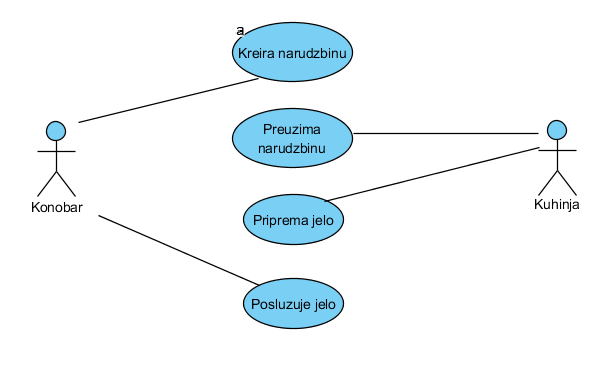
\includegraphics[width=\textwidth]{SU_7_konobar_kuhinja.png}
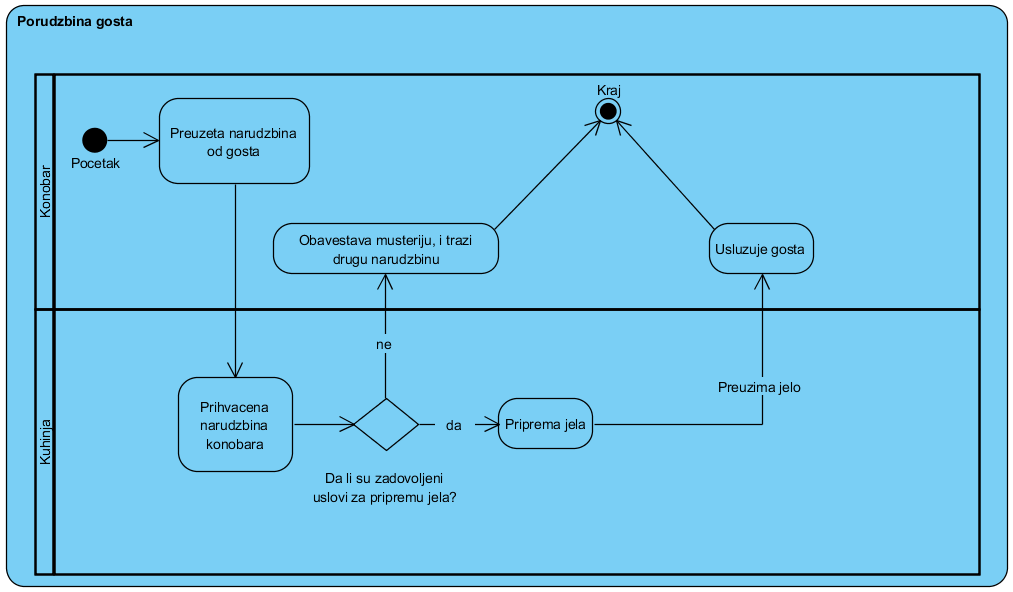
\includegraphics[width=\textwidth]{SU_7_porudzbina.png}

%%%%%%%%%%%%%%%%%%%%%%%%%%%%%%%%%%%%%%%%%%%%%%%%%%%%%%%%%%%%%%%%%%%%%%%%%%%%

\section{Baza podataka}

%%%%%%%%%%%%%%%%%%%%%%%%%%%%%%%%%%%%%%%%%%%%%%%%%%%%%%%%%%%%%%%%%%%%%%%%%%%%

\section{Predlog korisničkog interfejsa}

%%%%%%%%%%%%%%%%%%%%%%%%%%%%%%%%%%%%%%%%%%%%%%%%%%%%%%%%%%%%%%%%%%%%%%%%%%%%

\section{Prototip}

%%%%%%%%%%%%%%%%%%%%%%%%%%%%%%%%%%%%%%%%%%%%%%%%%%%%%%%%%%%%%%%%%%%%%%%%%%%%

\end{document}
